\documentclass[final]{article}

\usepackage{neurips_2024}

\usepackage[utf8]{inputenc}
\usepackage[T1]{fontenc}
\usepackage{amsmath,amsfonts,amssymb}
\usepackage{graphicx}
\usepackage{booktabs}
\usepackage{float}
\usepackage[round,authoryear]{natbib}
\usepackage[hidelinks,unicode=true]{hyperref}
\usepackage{url}
\usepackage{xcolor}
\usepackage{multirow}
\usepackage{array}

\title{Circuits Are Basis-Dependent Computations:\\
Transplantation Failure and Rescue Across\\
Task-Matched Networks}

\author{%
  Jack Large\\
  \texttt{jlarge6@student.cccs.edu}
}

\begin{document}

\maketitle

%-----------------------------------------------------------------------
\begin{abstract}
Mechanistic interpretability typically treats \emph{circuits}---identifiable
subgraphs of attention heads and MLP neurons---as the fundamental units of
transformer computation. This framing implicitly suggests circuits should be
portable: a head that implements induction in one network should, in principle,
be transplantable into another network trained on the same task. We
show that direct transplantation fails but is not an absolute impossibility:
compatibility can be learned by the host or supplied by sufficiently broad
residual-stream adapters. Across 20 independently trained small transformers
that all converge on Layer-0 induction circuits (Layer 0 is critical in 20/20
seeds; head-level agreement 23.2\%, 95\% CI [17.4\%, 29.5\%], $p=0.002$ vs.\
uniform null), moving a known-functional critical head into another network's
critical slot drops accuracy from 0.964 to 0.095, indistinguishable from
randomized controls. Two-interface Procrustes alignment reaches 0.084 despite
improving residual-stream $R^2$, and a seven-method head-interface alignment
tournament does not rescue the transplant. However, two rescue experiments
change the interpretation: freezing the transplanted donor head and retraining
the host recovers $\geq 80\%$ of recipient baseline in 100--500 steps across
five seed pairs---0.5--2.5\% of the original 20,000-step training
budget---and four residual-stream adapters recover 0.956--0.960 accuracy with
the recipient otherwise frozen. Joint training can force
post-L0/post-L1 CKA above 0.99 while raw head transplantation still fails,
showing that global residual similarity is insufficient. Scale probes sharpen
the boundary conditions: at 19M parameters on character-level Shakespeare,
slot-matched single-head transplant largely preserves performance, but after
ablating an average of four redundant L0 heads while preserving the recipient's
critical slot, transplanting into that slot drops 0.445 advantage; in
Pythia-160M, unaligned and Procrustes selected-head transplants both remain
below recipient baseline, while broad adapters solve the synthetic probe
equally well with the donor head zeroed. We therefore propose a narrower claim:
circuits are basis-dependent computations. The computation can recur across
training runs, but raw weights are not portable without a learned compatibility
map, and broad adapters must be controlled for task learning independent of the
donor component.
\end{abstract}

%-----------------------------------------------------------------------
\section{Introduction}
\label{sec:intro}

A circuit, in current interpretability practice, is a set of weights---specific
attention heads, specific neurons---that implement an identifiable computation.
The induction circuit \citep{olsson2022induction} is two heads: a
previous-token head in one layer and a content-matching head in a later layer.
The IOI circuit \citep{wang2023ioi} is 26 labeled components. Sparse feature
circuits \citep{marks2024sparse} are selected subgraphs of interpretable SAE
features. In each case, the circuit is named in terms of its \emph{components}.
The implicit claim is that those components carry the computation.

This paper asks whether that claim is literally true. If a circuit is its
components, then transplanting the components should preserve the behavior those
components support. We
test this directly: we train small transformers from scratch on content-matching
induction, identify each model's critical head via surgical ablation, and move a
known-functional head from one network into another network's critical slot.
As a raw weight operation, the transplant fails. Performance drops from
${\sim}96\%$ to ${\sim}9\%$, no better than inserting shuffled weights and
near the same receiving model with the critical head zeroed. The failure is
not absolute: later rescue experiments show that the recipient can learn to
use the donor head after 100--500 host-retraining steps---0.5--2.5\% of the
original 20,000-step training budget---and that broad residual-stream adapters
can restore ${\sim}96\%$ accuracy with the recipient otherwise frozen. The
negative result is therefore not that circuits are
indivisible below network scale, but that raw circuit weights are not portable
without an accompanying compatibility map.

This failure happens even though the two networks are trained on the same
deterministic task and converge on the same aggregate circuit motif. Our
seed-divergence experiments on 20 independently trained content-matching
induction models show that every seed develops a critical induction head in
Layer 0 (20/20 layer agreement), but the specific head varies across seeds
(23.2\% head-level agreement, $p=0.002$ vs uniform null). The networks agree on
the \emph{what} (induction via an L0 head); they disagree on
the \emph{where} (which head within L0); and they encode the \emph{how} in
ways that are not mutually portable.

We argue this forces a conceptual revision: \textbf{circuits are not raw
components but basis-dependent computations}. The computation is a stable
attractor of the training dynamics---reproducible across initializations,
developmentally ordered, and predictable under task changes. Its implementation
in weights depends on the residual-stream interfaces those weights read from
and write to. A head's ``function'' is not a property of the head alone; it is a
property of the head-plus-basis system, and that system can sometimes be
reconnected by learned adapters or retraining.

An implementation analogy is closer than a linguistic one. A compiled
instruction sequence can implement the same algorithm under two register
allocations, but a copied instruction is only meaningful relative to the
register state, calling convention, and memory layout it was compiled against.
Moving it into a program compiled under a different convention need not move the
computation; it may simply read the wrong registers. A compatibility shim or
brief recompilation can make the code usable again. Our finding is that circuit
weights stand in an analogous relation to their host network: they carry
computational content, but only when read by the residual-stream basis and
downstream interfaces they were trained alongside.

This has immediate implications. First, it dissolves an apparent tension in the
universality literature: \citet{lan2025universal} find feature spaces universal
across architectures, while \citet{bali2026headstability} find individual heads
unstable across seeds. Both are correct at different levels: the feature space
is the basis; the individual head is a basis-specific instrument. Second, it
constrains interpretability tooling: tools that extract ``circuits'' as portable
units are describing a computation, not excerpting a reusable module. Third, it
reframes questions in alignment and model editing: modifying ``the safety
circuit'' requires compatibility with the host basis, not just a locally
identified set of safety-relevant weights.

The paper develops these claims as follows. Section~\ref{sec:related} reviews
prior work on circuit universality and identifies the gap our paired measurement
fills. Section~\ref{sec:methods} describes methods, including a correction to
the standard \texttt{pos\_dep} metric. Section~\ref{sec:transplant} presents
the transplantation result. Section~\ref{sec:universality} documents the
functional universality that makes the transplantation result puzzling.
Sections~\ref{sec:taskarch}--\ref{sec:depth} present three supporting findings.
Section~\ref{sec:nlp} addresses natural-language generalization.
Section~\ref{sec:discussion} discusses implications. Section~\ref{sec:limits}
is limitations.

\paragraph{Summary of contributions.}
\begin{enumerate}
\item \textbf{Transplantation failure and rescue:} A known-functional head
      transplanted into the functionally-equivalent critical slot of another
      network performs no better than random weights, while host retraining and
      multi-interface residual adapters can recover performance
      (Section~\ref{sec:transplant}).
\item \textbf{Paired measurement of functional vs.\ structural universality:}
      100\% layer-level agreement with 23.2\% head-level agreement across 20
      seeds trained from scratch on the same content-matching induction task
      (Section~\ref{sec:universality}).
\item \textbf{Task structure determines architecture:} Three distinct regimes
      selected by task statistics, with a binary attention-engagement threshold
      at zero task entropy (Section~\ref{sec:taskarch}).
\item \textbf{Universal developmental order:} OV (output capacity) reliably
      precedes QK (routing capacity) across seeds and regimes
      (Section~\ref{sec:devorder}).
\item \textbf{Scale and divergence probes:} Shared-trajectory, shared-basis,
      19M Shakespeare, and Pythia-160M probes show that portability depends on
      training history, interface choice, and scale/task regime
      (Sections~\ref{sec:transplant}--\ref{sec:scale}).
\item \textbf{Depth-scaling trend for suppression cascades:} Layer 0 composition
      is invariant; suppression scales linearly with depth
      (Section~\ref{sec:depth}).
\item \textbf{Synthetic-to-natural generalization:} Circuits identified on
      synthetic tasks predict in-context copying behavior on real language
      (Section~\ref{sec:nlp}).
\item \textbf{Methodological correction:} Permutation-sensitivity resolves
      39/48 false-positive ``positional'' classifications in our Shakespeare
      model (Section~\ref{sec:methods}).
\end{enumerate}

%-----------------------------------------------------------------------
\section{Related Work}
\label{sec:related}

Our findings touch several active threads in mechanistic interpretability. We
organize related work into four categories.

\subsection{Circuit discovery and universality}

\paragraph{Canonical circuit motifs.}
The induction circuit of \citet{olsson2022induction} established the template
for circuit analysis: a two-head composition (previous-token head +
content-matching induction head) implementing in-context copying. The IOI
circuit in GPT-2 \citep{wang2023ioi} extended this to a 26-component circuit
with name-movers, backup heads, and inhibition heads. Attribution graphs
\citep{ameisen2025attribution} identify multi-hop reasoning and refusal circuits
in Claude 3.5 Haiku. Our work uses the induction circuit as a testbed but asks
a different question: not \emph{what} the circuit is, but \emph{what it means
for a circuit to ``be'' something} if the components that implement it are not
portable.

\paragraph{Cross-seed universality.}
\citet{gurnee2024universal} analyzed neuron identity across 5 GPT-2 models
trained from different seeds, finding only 1--5\% of neurons are ``universal.''
\citet{nandan2025universal} extended this with training checkpoints, showing
universal neurons emerge early and persist. Our work operates at the head level
and documents a structurally analogous finding: at the component level, only
${\sim}13\%$ of seeds share critical-head identity.

\paragraph{Cross-architecture universality.}
\citet{wang2024transformers} compared induction circuits in Transformers and
Mambas, finding structurally analogous circuits. \citet{lan2025universal}
formalized ``analogous feature universality'' across language models: SAE
feature spaces are similar across architectures under rotation-invariant
transforms. Our work complements these by measuring universality \emph{within}
architecture across seeds, and by demonstrating that universality holds at the
algorithm level but not at the weight level.

\paragraph{Cross-seed instability.}
\citet{bali2026headstability} measured attention-head stability across training
runs, finding that middle-layer heads are particularly unstable (cosine
similarity ${\sim}0.70$). This appeared in tension with the Lan/Wang
universality results. Our paper resolves this tension: feature spaces can be
universal at the basis level while individual heads are unstable at the
component level. Both findings are correct at different levels of description.

\paragraph{The gap our work fills.}
Prior work has not, to our knowledge, paired functional circuit recurrence with
direct weight-portability tests in the same controlled setting. Our
transplantation result directly tests whether circuit weights can be moved
across independently trained networks that solve the same task.

\subsection{Circuit formation dynamics}

\paragraph{Grokking.}
The grokking phenomenon---delayed generalization long after training loss
converges---has been studied extensively since \citet{power2022grokking}.
\citet{nanda2023grokking} identified grokking as circuit formation with
weight-decay-driven cleanup of a memorization circuit.
\citet{varma2023grokking} formalized this as circuit efficiency competition.
Our grokking-like transition in content-matching induction differs---the model
is at near-chance throughout the pre-transition period---matching
\citet{kumar2024lazyrich}'s ``lazy-to-rich'' transition framing.

\paragraph{Induction head emergence.}
\citet{olsson2022induction} documented a sharp phase change in in-context
learning coinciding with induction head formation. \citet{singh2024induction}
decomposed this into subcircuit maturation: QK match, OV copy, and positional
previous-token copier must all mature simultaneously. \citet{edelman2024evolution}
document a ``unigram plateau'' before bigram induction emerges, providing the
closest prior analogue to our pre-transition plateau.

\paragraph{Our contribution.}
The ``hardware before software'' ordering---OV developing reliably before QK,
with a 12,000-step separation in the grokking regime---has not been previously
documented. \citet{singh2024induction} measure subcircuit timing but do not
emphasize the \emph{ordering} as a universal feature. Our per-metric
crystallization analysis provides a finer-grained view of what happens during
consolidation.

\subsection{Task-dependent algorithm selection}

\citet{kawata2025shortcut} proved via gradient-flow analysis that data diversity
determines whether a transformer adopts a positional shortcut or a
content-matching induction head. Their result is theoretical; ours is empirical
and extends to a third regime (the suppression cascade in natural-language
tasks). \citet{rende2024simplicity} document a ``distributional simplicity
bias'': low-order token interactions are learned before high-order ones.
\citet{minegishi2025beyond} report that in-context meta-learning tasks produce
multiple training phases, each with a qualitatively distinct circuit.

\subsection{Methodological work}

Standard practice classifies attention heads by pattern statistics. Our
methodological audit identifies a pitfall: the cross-input consistency metric
has a high false-positive rate in deeper layers, because the residual stream has
already encoded rich content information, and content-conditional attention can
appear pattern-stable. We introduce permutation-sensitivity as a more reliable
content-vs-position classifier. \citet{mcdougall2024copysuppression} identified
a specific copy-suppression head in GPT-2 Small. Our Shakespeare model exhibits
suppression as the \emph{dominant} motif (39/48 heads at depth 6), extending
their single-head characterization to a layer-by-layer scaling analysis.
Causal attribution follows \citet{meng2022activation} and \citet{wang2023ioi}.

%-----------------------------------------------------------------------
\section{Methods}
\label{sec:methods}

\subsection{Architecture and training}

All small-scale experiments use a GPT-2-style decoder-only transformer.
Ablation robustness studies use 2-layer, 4-head, 128-dimensional models
(${\sim}460$K parameters). The natural-language Shakespeare model uses 6 layers,
8 heads, and 512-dimensional residual stream (${\sim}19$M parameters, trained
character-level). Training uses AdamW with cosine schedule; dense checkpoints
are saved every 25--100 steps. Full hyperparameter details are in
Appendix~\ref{app:methods}.

\subsection{Tasks}

We study five task families: (1)~\textbf{Positional induction}---repeated-sequence
copy where the correct token is always at a fixed positional offset; (2)~\textbf{Content-matching
induction}---random-position bigrams forcing token-identity matching (vocab=512,
no positional shortcut); (3)~\textbf{Markov chain}---next-token prediction under
varying entropy levels (H=0.0 to H=1.0, vocab=64); (4)~\textbf{IOI}---indirect
object identification; (5)~\textbf{Natural language}---character-level prediction
on TinyShakespeare (1.1M characters, 65-char vocabulary).

\subsection{Circuit extraction}

We use three complementary methods:
\begin{itemize}
\item \textbf{Activation patching} \citep{meng2022activation}: patch a
      component's output from a clean run into a corrupted run; measure accuracy
      recovery. Components with large recovery are causally necessary.
\item \textbf{Head profiling}: compute per-head OV copy score (diagonal dominance
      of the OV circuit), QK content-matching score, and positional dependence
      ($\mathtt{pos\_dep}$, cross-input attention variance).
\item \textbf{Surgical ablation}: zero-out individual components and measure
      task accuracy drop. This identifies \emph{critical} components.
\end{itemize}

\subsection{Permutation-sensitivity metric (methodological correction)}
\label{sec:permtest}

The standard $\mathtt{pos\_dep}$ metric measures how much attention patterns
vary across inputs. Low variance implies a ``positional'' head. However, in
deeper layers the residual stream already encodes rich content, and
content-conditional attention can produce patterns that look cross-input-stable
to $\mathtt{pos\_dep}$.

We introduce \textbf{permutation sensitivity}: for each head, we measure the
$L_2$ distance between attention patterns on the original input and on the same
input with token identities randomly permuted while preserving positions. A
positional head is unaffected by token permutation; a content-based head is
not. On our Shakespeare model (48 heads), $\mathtt{pos\_dep}$ classifies 47/48
heads as positional; permutation sensitivity classifies 9/48 as positional,
resolving 39 false positives. These 39 heads are content-based suppressors in
layers 1--5. On our entropy=0 model, both metrics agree (16/16 positional), as
expected when attention is genuinely positional.

%-----------------------------------------------------------------------
\section{Transplantation Failure}
\label{sec:transplant}

\subsection{Setup}

We train two independent instances of a 2-layer content-matching induction
model (seeds 0 and 1), each converged to high accuracy. We identify the
``critical head''---the single head whose ablation causes the largest accuracy
drop:
\begin{itemize}
\item \textbf{Seed 0:} L0H3 is critical. Ablation drops accuracy from 0.854 to
      0.041 ($-$0.813).
\item \textbf{Seed 1:} L0H1 is critical. Ablation drops accuracy from 0.964 to
      0.118 ($-$0.846).
\end{itemize}
Both networks solve the same content-matching task via a single dominant L0
head, but \emph{which} head differs. This is the paradigm case of functional
recurrence with contingent wiring: same task and circuit motif, different
component.

\begin{figure}[H]
  \centering
  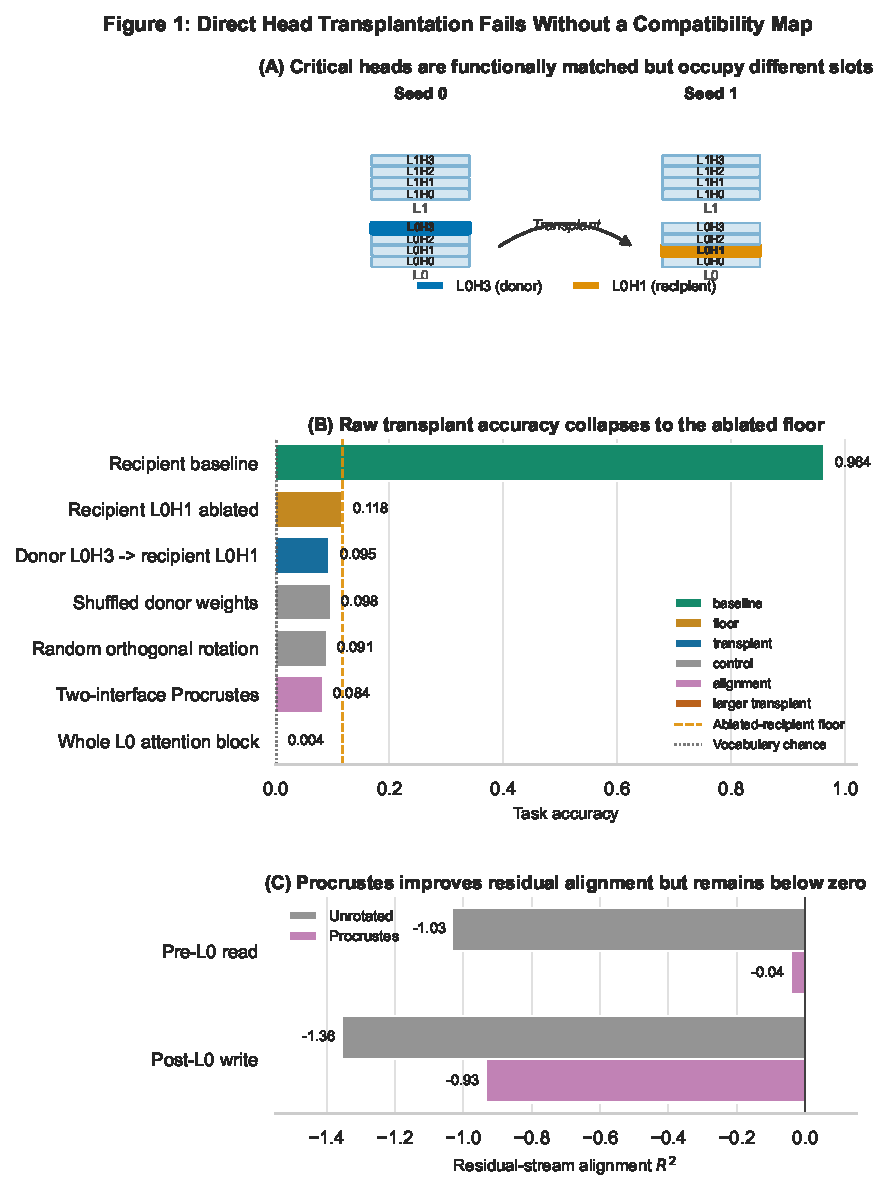
\includegraphics[width=\textwidth,height=0.72\textheight,keepaspectratio]{figures/fig1_transplantation.pdf}
  \caption{\textbf{Direct head weights are not portable across independently
  trained task-matched networks.} Two small transformers (seeds 0 and 1) both converge on induction
  circuits that cause accuracy drops of 0.81 and 0.85 when their critical Layer
  0 heads are ablated. Across 20 seeds of this task, 100\% of seeds place their
  critical head in Layer 0 (head-level agreement 23.2\%, $p=0.002$). \textbf{Yet the weights are not transplantable:} moving seed
  0's critical head (L0H3) into seed 1's critical slot (L0H1) drops accuracy
  from 0.964 to 0.095---indistinguishable from shuffled random weights (0.098)
  or a random orthogonal rotation (0.091). Two-interface Procrustes alignment
  provides no rescue (0.084), even though alignment measurably improves the
  residual-stream match (pre-L0 $R^2$ improves from $-1.03$ unrotated to
  $-0.04$ aligned). Improved basis alignment does not recover function.}
  \label{fig:transplant}
\end{figure}

\subsection{The transplantation test}

We extract seed 0's L0H3 Q/K/V projections and output projection columns, and
insert them into seed 1's L0H1 slot. If head weights are carriers of function,
seed 1's induction capability should be preserved.

\subsection{Results}

Table~\ref{tab:transplant} shows results. The functional head transplant
produces the same performance as random weights. Three controls confirm this is
not an artifact: inserting seed 0's non-critical head is equally bad; inserting
shuffled weights is equally bad; and a clean-slate replacement (ablate then
insert) recovers nothing.

\begin{table}[h]
\centering
\caption{Transplantation results. The functional head is not portable.}
\label{tab:transplant}
\begin{tabular}{lcc}
\toprule
Configuration & Accuracy & $\Delta$ vs.\ seed 1 baseline \\
\midrule
Seed 1 baseline                                          & 0.964 & --- \\
Seed 1 with L0H1 ablated                                 & 0.118 & $-$0.846 \\
\textbf{Seed 0's L0H3 $\to$ seed 1's L0H1 (critical slot)} & \textbf{0.095} & $-$0.869 \\
Seed 0's L0H3 $\to$ seed 1's L0H3 (non-critical slot)   & 0.966 & $+$0.002 \\
Seed 0's non-critical head $\to$ seed 1's L0H1 (ctrl A) & 0.100 & $-$0.864 \\
Shuffled random weights $\to$ seed 1's L0H1 (ctrl B)    & 0.098 & $-$0.866 \\
\bottomrule
\end{tabular}
\end{table}

\subsection{What this rules out}

This result rules out a family of explanations:
\begin{itemize}
\item \emph{``Both networks learned the same weights''} --- directly falsified;
      transplant would succeed.
\item \emph{``Same weights up to permutation''} --- if so, aligning to the
      correct head-identity permutation would work. It doesn't.
\item \emph{``The circuit lives in a few specific weights''} --- if so, those
      weights would be transplantable. They aren't.
\end{itemize}
What remains: the function is encoded in the \emph{interaction} between the
critical head's weights and the residual stream basis that surrounds them---a
basis shaped by every other weight in the network.

\subsection{Basis alignment does not rescue transplantation}

We test whether the two task-matched networks encode the relevant computation in
rotated bases using \emph{two-interface Procrustes alignment}: the donor head's
Q/K/V projections read from the pre-L0 LayerNorm interface, while its output
projection writes into the post-L0 residual interface --- these are different
subspaces and require separate alignment. We collect activations at both
interfaces from both networks on identical inputs, compute the orthogonal
rotations $R_{\mathrm{in}} = \arg\min_R \|X_{\text{seed0}}^{\mathrm{pre}} R -
X_{\text{seed1}}^{\mathrm{pre}}\|_F$ and analogously $R_{\mathrm{out}}$ at the
post-L0 interface, apply $R_{\mathrm{in}}$ to the donor's Q/K/V rows and
$R_{\mathrm{out}}^\top$ to its output-projection columns, then transplant.

\begin{table}[h]
\centering
\caption{Procrustes alignment does not rescue the transplant.}
\label{tab:procrustes}
\begin{tabular}{lcc}
\toprule
Configuration & Accuracy & $\Delta$ vs.\ seed 1 baseline \\
\midrule
Unaligned transplant               & 0.095 & $-$0.869 \\
One-interface aligned (post-L0 only)   & 0.094 & $-$0.870 \\
\textbf{Two-interface aligned (corrected)} & \textbf{0.084} & \textbf{$-$0.880} \\
Random rotation control            & 0.091 & $-$0.873 \\
Aligned non-critical donor         & 0.107 & $-$0.857 \\
\bottomrule
\end{tabular}
\end{table}

Alignment produces no rescue. Paired sign-flip tests on the 1024 fixed eval
sequences (per-sequence accuracy differences) yield: unaligned vs.\
two-interface aligned mean diff $= -0.011$, $p=0.003$ --- the aligned
transplant is in fact \emph{significantly worse} than unaligned, not better.
Unaligned vs.\ one-interface aligned is indistinguishable ($p=0.73$), and
unaligned vs.\ random rotation is indistinguishable ($p=0.20$). All
transplant conditions are far below baseline (0.964) and cluster near the
ablated-head floor ($\approx 0.09$ on 1024 sequences, indistinguishable from
simply zeroing the recipient's L0H1 with no replacement at 0.118). This is
catastrophic failure relative to the functional model, but it is not
vocabulary-chance (which is $1/512 \approx 0.002$); the transplanted weights
contribute a small amount of residual signal that the recipient network's
downstream components cannot usefully read.

Importantly, the two-interface alignment \emph{does} find a substantially
better basis match than no rotation: the pre-L0 read-interface Procrustes
improves $R^2$ from $-1.03$ (unrotated) to $-0.04$ (aligned), and the post-L0
write-interface improves from $-1.36$ to $-0.93$. Despite finding a measurably
better basis, the transplant accuracy does not recover --- if anything, the
alignment slightly hurts.

\paragraph{Alignment tournament.}
To rule out the possibility that the transplant failure is peculiar to
orthogonal rotations, we run a tournament of seven alignment methods on the
same seed 0 $\to$ seed 1 transplant (Table~\ref{tab:alignment_tournament}):
(1) Unaligned; (2) Procrustes orthogonal (two-interface); (3) Affine
(orthogonal + per-axis scale, no translation since model is bias-free);
(4) CKA-optimized linear map (unconstrained linear $A$ maximizing linear CKA
between aligned activations, initialized from Procrustes $R$); (5) Git Re-Basin
style weight-permutation matching \citep{ainsworth2022git} applied to the 4
attention heads and 512 MLP units per layer, then composed with Procrustes;
(6) Learned linear adapter (two $d \times d$ matrices trained on induction
loss with all other weights frozen, 1000 AdamW steps); (7) Learned nonlinear
adapter (2-layer MLP with hidden width $4d$ at each interface, same training
protocol).

\begin{table}[h]
\centering
\small
\caption{Head-interface alignment tournament. No head-local method rescues the
transplant. Learned
nonlinear adapter reaches 0.118 only because it learns to \emph{ignore} the
donor head (matches donor-zero control at 0.1178).}
\label{tab:alignment_tournament}
\begin{tabular}{lccc}
\toprule
Method & Accuracy & $\Delta$ vs.\ unaligned & Paired $p$-value \\
\midrule
Unaligned (baseline) & 0.0951 & --- & --- \\
Procrustes (two-interface) & 0.0838 & $-$0.0112 & 0.003 \\
Affine (orthogonal + scale) & 0.0780 & $-$0.0171 & $<$0.001 \\
CKA-optimized linear map & 0.0981 & $+$0.0031 & 0.37 \\
Git Re-Basin + Procrustes & 0.0838 & $-$0.0112 & 0.003 \\
Learned linear adapter & 0.0951 & $+$0.0000 & 1.00 \\
\textbf{Learned nonlinear adapter} & \textbf{0.1180} & $+$0.0229 & $<$0.001 \\
\midrule
\emph{Control: donor head zeroed, adapter only} & 0.1178 & $+$0.0228 & $<$0.001 \\
\bottomrule
\end{tabular}
\end{table}

Every alignment method produces accuracy below 0.12, compared to the seed 1
baseline of 0.964. More importantly, the only method that nominally
``improves'' on unaligned --- the learned nonlinear adapter, reaching 0.1180
--- matches the donor-zero control (0.1178) within noise. That is, the
2-layer nonlinear adapter learned to \emph{null out} the donor head entirely;
its apparent improvement is explained by the adapter bypassing the donor, not
by alignment recovering donor function. The learned linear adapter, lacking
the capacity to zero-out the donor subspace, stayed at exact unaligned
performance ($p=1.0$).

\paragraph{What the tournament rules out.}
A sophisticated reader might object that orthogonal alignment is the narrowest
family of transforms, and non-portability could be corrected by more
expressive alignments. Our tournament tests the four largest expressivity
tiers at the donor head's read/write interface: orthogonal (Procrustes),
orthogonal + scale (affine), unconstrained linear (CKA-optimized + learned
linear), and nonlinear ($4d$-width MLP adapters). \textbf{None of these
head-local maps rescues the transplant.} The only method that moved above
unaligned did so by learning to ignore the donor. This narrows the failure:
the problem is not corrected by a local change of basis at the transplanted
head's two interfaces.

\subsection{Rescue by host retraining and multi-interface adapters}
\label{sec:rescue}

The head-interface tournament rules out a narrow family of alignment fixes; it
does not show that the donor head contains no usable computation. We therefore
run two rescue experiments.

First, we transplant the donor critical head into the recipient critical slot,
freeze the transplanted head, and retrain every other recipient parameter. For
five donor-recipient pairs, the recipient recovers at least 80\% of its original
baseline within 100--500 retraining steps, compared with the original 20,000
training-step budget (Table~\ref{tab:partial_retrain}). Thus the donor head
carries useful structure, but the surrounding network must learn how to read it.
The ratio is the important quantity: the host learns the compatibility map in
0.5--2.5\% of the original training budget, so the function is close to usable
but not expressed in the recipient's native basis.

\begin{table}[h]
\centering
\caption{Partial-retraining rescue. After transplanting the donor head and
freezing it, the host recovers $\geq 80\%$ of recipient baseline in 100--500
steps, 0.5--2.5\% of the original 20,000-step budget.}
\label{tab:partial_retrain}
\begin{tabular}{lcccc}
\toprule
Pair & Recipient baseline & Zero-head control & Final accuracy & $K^\star$ \\
\midrule
0$\to$1 & 0.9640 & 0.1178 & 0.9648 & 100 \\
0$\to$3 & 0.9629 & 0.4611 & 0.9614 & 100 \\
1$\to$4 & 0.9621 & 0.0586 & 0.9629 & 100 \\
3$\to$5 & 0.9618 & 0.0299 & 0.9627 & 500 \\
4$\to$6 & 0.9606 & 0.7824 & 0.9583 & 100 \\
\bottomrule
\end{tabular}
\end{table}

Second, we freeze the recipient and train adapters only. A single post-L0
linear adapter improves accuracy from 0.0951 to 0.4791 but does not recover
baseline. Four residual-stream adapters placed before the embedding stream,
after L0, after L1, and before the unembedding recover nearly all function:
0.9561 for linear adapters and 0.9601 for two-layer MLP adapters
(Table~\ref{tab:stitching_adapters}). The failure is therefore interface
coverage, not lack of any compatible computation in the donor weights.

\begin{table}[h]
\centering
\caption{Multi-interface adapter rescue. The recipient is frozen; only adapters
are trained for 2000 AdamW steps.}
\label{tab:stitching_adapters}
\begin{tabular}{lc}
\toprule
Condition & Accuracy \\
\midrule
Recipient baseline & 0.9640 \\
Bare transplant / no adapter & 0.0951 \\
Post-L0 linear adapter & 0.4791 \\
All-four linear adapters & 0.9561 \\
All-four MLP adapters & 0.9601 \\
\bottomrule
\end{tabular}
\end{table}

These rescues force a narrower interpretation of the negative transplant
result. Direct head transplantation and head-local alignment fail, but the
failure is not proof that the head is functionally arbitrary. The relevant unit
is the donor computation together with enough learned interface machinery for
the host to read and write in the donor-compatible basis.

\paragraph{Residual stream geometry: distinct manifolds, not rotations.}
To ground the ``basis matters'' claim geometrically, we compute pairwise
linear-CKA across all 20 seeds' residual stream activations at three
interfaces (pre-L0-LN, post-L0, post-L1) on the same 1024-sequence fixed eval
set. Mean pairwise CKA is $0.013$ at pre-L0 and $0.006$ at post-L0 --- seeds
occupy almost entirely disjoint linear subspaces in the residual stream.
Critically, pairwise CKA is \emph{uncorrelated} with shared critical-head
identity (Pearson $r=-0.03$, $p=0.67$, $n=190$), and the mean CKA for seed
pairs that share the same critical-head slot is $0.013$, identical to the
mean for pairs that do not. This supports the stronger reading of the
transplantation result: the 20 seeds compute a shared algorithm over genuinely
distinct manifolds that are not related by any linear isometry. Alignment
fails not because the rotation we tried was wrong but because there is no
rotation that brings the manifolds into coincidence.

\subsection{Static partial transplants require large compatible context}

Table~\ref{tab:wholenet} shows the results of progressively larger transplants.
Every static partial transplant fails catastrophically. The single-head transplant
stays at ${\sim}9.5\%$ accuracy (near the baseline-with-head-ablated level of
$11.8\%$). All \emph{larger} partial transplants (whole attention block through
all-weights-except-L1-block) drop even lower, to ${\sim}0.4$--$1.2\%$ accuracy
--- at or just above the random-chance floor ($1/512 \approx 0.002$) ---
indicating near-complete loss of induction function. Only the full transplant
recovers seed 0's accuracy when no adapter or retraining is allowed.

\begin{table}[h]
\centering
\caption{Static partial-transplant study. Every fixed partial scope tested
fails catastrophically without learned compatibility machinery; full-network
transplant recovers function. See Sections~\ref{sec:rescue} and
\ref{sec:minunit} for rescue and finer-grained characterizations.}
\label{tab:wholenet}
\begin{tabular}{lc}
\toprule
Transplant scope & Accuracy \\
\midrule
Single-head L0H3 $\to$ L0H1                          & 0.095 \\
Whole L0 attention block (all 4 heads)               & 0.004 \\
Whole L0 block (attention + MLP + LayerNorms)        & 0.005 \\
Whole L0 block + final LayerNorm                     & 0.006 \\
Embeddings only                                       & 0.012 \\
Embeddings + L0 attention                            & 0.004 \\
Embeddings + L0 full block                           & 0.007 \\
All weights except L1 block                          & 0.007 \\
\textbf{Full transplant (all 15 weights)}            & \textbf{0.861} \\
\bottomrule
\end{tabular}
\end{table}

The most striking case is ``all weights except L1 block'': we transplant seed
0's embeddings, L0 attention, L0 MLP, L0 LayerNorms, and final LayerNorm,
leaving only seed 1's L1 block intact. Accuracy: 0.007. Seed 0's L0 writes
into a representational basis that seed 1's L1 cannot read. This reveals tight
coupling between adjacent learned interfaces. The adapter results in
Section~\ref{sec:rescue} show that this coupling can be bridged by learned
maps, but the bridge is not present in the raw partial transplant.

\subsection{Minimum functional unit: a finer-grained characterization}
\label{sec:minunit}

Table~\ref{tab:wholenet} tests a handful of structured partitions; it does not
localize precisely where function breaks. We run a systematic sweep across all
15 weight tensors in the 2-layer model to answer: \emph{which single tensor,
when transplanted, breaks the recipient?} and \emph{what is the smallest
subset whose transplant preserves accuracy $\geq 0.5$?}

\begin{table}[h]
\centering
\caption{Per-tensor single-transplant sweep. Attention Q/K/V/O projections are
individually disruptive; LayerNorms and most MLP projections transplant
without breaking recipient function.}
\label{tab:minunit_sweep}
\begin{tabular}{lc}
\toprule
Single-tensor transplant $\to$ seed 1 & Accuracy \\
\midrule
L0 attention qkv\_proj alone  & 0.006 \\
L0 attention out\_proj alone  & 0.002 \\
L1 attention qkv\_proj alone  & 0.001 \\
L1 attention out\_proj alone  & 0.002 \\
L0 MLP up\_proj alone         & 0.948 \\
L0 MLP down\_proj alone       & 0.958 \\
L0 LayerNorm (ln1/ln2) alone  & 0.963--0.965 \\
All LayerNorms together       & 0.963 \\
L1 MLP (up+down) together     & 0.962 \\
L0 MLP (up+down) together     & 0.324 \\
wte (token embedding) alone   & 0.796 \\
\midrule
Greedy peel-back minimum (9 of 15 tensors, 72\% of params) & 0.593 \\
\bottomrule
\end{tabular}
\end{table}

Two observations. First, the \emph{break-unit} is surprisingly small: a single
attention projection matrix ($\sim$3--10\% of parameters), transplanted alone,
drops accuracy from 0.964 to 0.001--0.006. Second, the \emph{static
rescue-unit} is large under this heuristic: the greedy peel-back, starting from
all 15 tensors and removing those that can be removed while keeping accuracy
$\geq 0.5$, stops at 9 tensors (72\% of parameters). This is a local greedy
solution, not an exhaustive lower bound over all $2^{15}$ tensor subsets. It
shows that a large compatible context is sufficient and that every single
tested attention projection is disruptive on its own; it does not prove that no
smaller non-greedy subset exists.

These two observations are consistent: Q/K/V/O projections are the components
most tightly co-adapted, and the rescue set needs enough of them plus their
surrounding weights to produce functional output. The minimum static
transplant unit is \emph{not} the whole network, but it is substantially larger
than the head-level or attention-block-level scales assumed by
circuit-extraction methodology. Learned adapters reduce the amount of donor
weight context needed by supplying a compatibility map instead of copying more
of the donor network.

\subsection{Training-time portability: when does non-portability emerge?}
\label{sec:portability_curve}

We use seed 0's 46 intermediate checkpoints (step $0$ to $20{,}000$ at 500-step
intervals) to ask when during training non-portability emerges. At each
checkpoint we transplant the donor's L0H3 into a fully-trained seed 1's L0H1
slot, both unaligned and two-interface-aligned.

\begin{figure}[H]
  \centering
  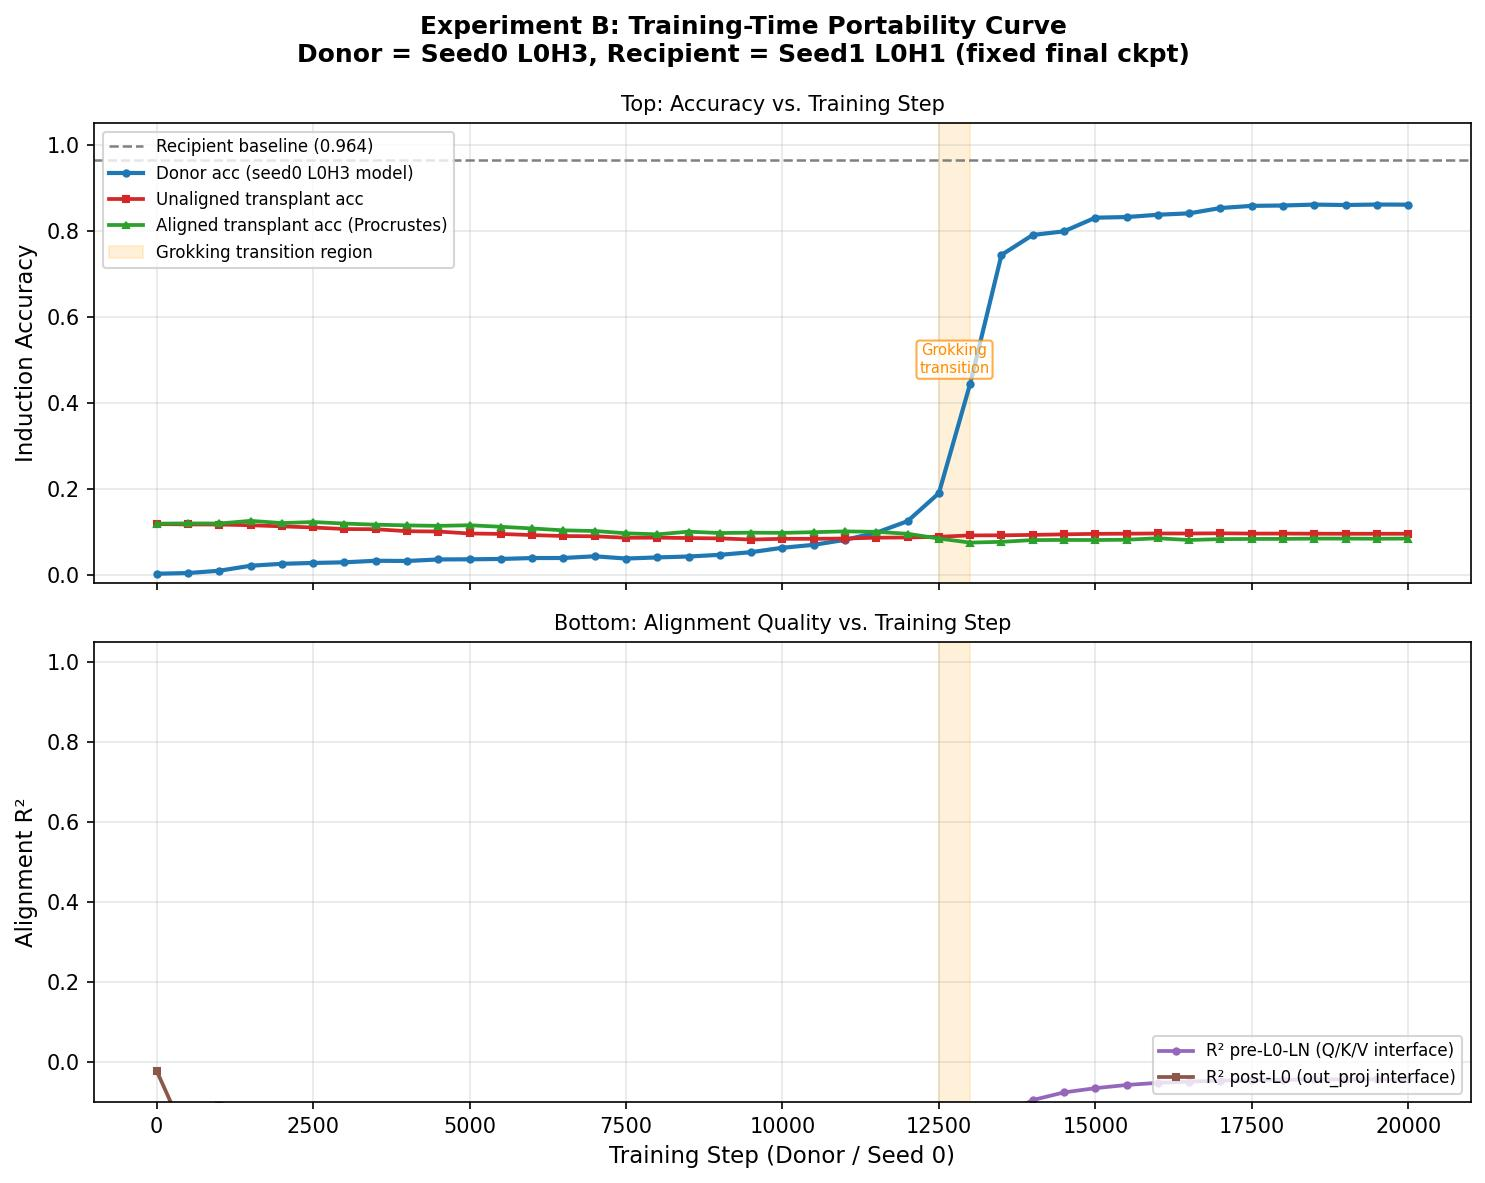
\includegraphics[width=0.9\textwidth]{figures/fig_portability_curve.pdf}
  \caption{\textbf{Fixed-recipient transplant accuracy is constant across donor training.} Donor accuracy
  (blue) rises from chance at step 0 to 0.86 at step 20{,}000, with a sharp
  grokking transition around step 12{,}500. Transplant accuracy (red/green,
  unaligned/aligned) stays at $\sim 0.09$--$0.12$ throughout --- both before
  the donor learns anything useful AND after it converges. The function and
  its basis co-develop: the donor's weights are non-portable from the very
  first training step at which they begin to encode function.}
  \label{fig:portability_curve}
\end{figure}

The transplant accuracy is essentially constant across training
($\sim 0.08$--$0.12$), regardless of whether the donor is random (step 0) or
fully converged (step 20{,}000). In this fixed-recipient checkpoint probe,
non-portability is not a slowly accumulating feature of late donor training.
From the moment the donor encodes anything useful, the encoding is
basis-specific relative to the fully trained recipient. The alignment
diagnostic $R^2$ evolves monotonically with training (pre-L0 $R^2$ from
$-0.65$ at step 0 to $-0.04$ at step 20{,}000), but this improved alignment
does not translate into any recovery of transplant function.

\subsection{Shared-trajectory forks}
\label{sec:sharedtrajectory}

The fixed-recipient checkpoint probe does not answer when two networks that
share early training history become transplant-incompatible. We therefore train
a shared prefix from a common initialization, fork into two data-order branches,
continue both branches to 20{,}000 steps, and transplant the critical head from
branch A into branch B.

\begin{table}[h]
\centering
\caption{Shared-trajectory transplant sweep. Values are means over three forked
pairs per fork point. The curve is not monotonic: compatibility is highest at
fork 500 and collapses for fork points 2000 and later.}
\label{tab:shared_trajectory}
\begin{tabular}{rccc}
\toprule
Shared steps before fork & Recipient baseline & Unaligned & Procrustes \\
\midrule
0 & 0.9634 & 0.3513 & 0.3467 \\
500 & 0.9610 & 0.6608 & 0.6572 \\
2{,}000 & 0.9598 & 0.0947 & 0.0936 \\
5{,}000 & 0.9587 & 0.0881 & 0.0875 \\
10{,}000 & 0.9593 & 0.0785 & 0.0782 \\
15{,}000 & 0.9604 & 0.0787 & 0.0787 \\
18{,}000 & 0.9635 & 0.0581 & 0.0582 \\
19{,}500 & 0.9625 & 0.0700 & 0.0700 \\
20{,}000 & 0.9613 & 0.0729 & 0.0729 \\
\bottomrule
\end{tabular}
\end{table}

The result is mixed rather than a simple decay curve. Forking after 500 shared
steps gives the strongest transplant compatibility, while fork points 2000 and
later mostly collapse near the ablated/transplant floor. This suggests that an
early compatibility window can exist, but the learned implementation becomes
branch-specific well before convergence. This does not contradict the
fixed-recipient checkpoint probe above: that probe asks whether a donor
checkpoint can be read by a fully trained independently initialized recipient,
while the fork sweep asks how long two branches that share initialization and
early optimization remain mutually readable. Together they localize the
commitment window. Compatibility is not gradually lost over the final training
phase; it is largely determined in the early interval after step 500 and before
step 2000, when the branch-specific implementation is selected.

\subsection{Shared-basis joint training}
\label{sec:sharedbasis}

We next test whether forcing residual-stream similarity is sufficient for
portability. Two models are trained jointly with an auxiliary loss
$\lambda(1-\mathrm{CKA})$ at post-L0 and post-L1 residual streams. All values
of $\lambda$ preserve task learning, and high $\lambda$ forces CKA above 0.99.
Raw transplantation still fails (Table~\ref{tab:shared_basis}).

\begin{table}[h]
\centering
\caption{Shared-basis joint training. High residual CKA does not make raw head
weights portable. Procrustes helps only partially at $\lambda=0.1$.}
\label{tab:shared_basis}
\begin{tabular}{rccccc}
\toprule
$\lambda$ & Baseline A & Baseline B & CKA post-L0/L1 & Unaligned & Procrustes \\
\midrule
0.00 & 0.9577 & 0.9637 & 0.0314 / 0.2783 & 0.1062 & 0.1066 \\
0.01 & 0.9613 & 0.9613 & 0.9223 / 0.9278 & 0.0597 & 0.0637 \\
0.10 & 0.9624 & 0.9627 & 0.9917 / 0.9982 & 0.0259 & 0.5049 \\
1.00 & 0.9574 & 0.9572 & 0.9992 / 0.9995 & 0.0184 & 0.1721 \\
\bottomrule
\end{tabular}
\end{table}

This rules out a simple version of the basis-mismatch explanation. Global
linear CKA can be made very high while the raw local head interface remains
incompatible. However, the $\lambda=0.1$ condition is not a pure null result:
combining high residual similarity with two-interface Procrustes raises
transplant accuracy to 0.5049, roughly halfway from the transplant floor to the
0.9627 recipient baseline. The non-monotonicity matters: $\lambda=1.0$ drives
CKA even higher (0.9992/0.9995) but lowers Procrustes transplant accuracy to
0.1721. The relevant compatibility relation is therefore more specific than
residual-stream similarity alone, and excessive CKA pressure may solve the
auxiliary objective in a way that removes the implementational flexibility that
made the $\lambda=0.1$ partial rescue possible.

%-----------------------------------------------------------------------
\section{Functional Universality Without Structural Universality}
\label{sec:universality}

The transplantation failure in Section~\ref{sec:transplant} is only puzzling
because the two networks solve the same task with the same coarse circuit motif.
We quantify this here.

\paragraph{Seed-divergence experiment.}
We train 20 independently initialized models on the content-matching induction
task (seeds 0--19, same architecture, same data). 19 of 20 seeds reach baseline
accuracy $>0.5$ within the standard 20{,}000-step budget; seed 2 remains on the
grokking plateau at 20k and was re-trained for 30{,}000 steps, after which it
also converged (final accuracy 0.966) --- see Appendix~\ref{app:results}. The
primary statistics report all 20 converged seeds on equal footing. For each
seed, we identify the critical attention head via single-head ablation and
measure pairwise alignment of the full 10-dimensional ablation effect vector
(8 heads + 2 MLPs) across 190 seed pairs. Head-level similarity: 0.329
(95\% CI [0.28, 0.38]). Layer-level agreement on the critical head:
\textbf{100\%} (20/20 seeds place the critical head in Layer 0). Head-level
agreement: \textbf{23.2\%} (95\% CI [17.4\%, 29.5\%], $p=0.002$ via
10{,}000-permutation test against the uniform null of 12.5\%).

\paragraph{Functional universality.}
Every seed develops a single critical L0 head with catastrophic ablation impact.
Across 4 seeds with full ablation robustness data (Appendix~\ref{app:ablation}):
mean accuracy drop = 0.775 $\pm$ 0.162 (95\% CI [0.59, 0.91]; $p=0.004$ vs.\
null of no impact).

\paragraph{Structural contingency.}
Despite functional universality, head-level agreement is only 23.2\% (95\% CI
[17.4\%, 29.5\%]; $p=0.002$ vs.\ random baseline of 12.5\%). No single
(layer, head) slot serves the critical role across all seeds.

\paragraph{Per-example agreement: matched accuracy is not behavioral equivalence.}
To test whether 20 networks that all hit ${\sim}96\%$ accuracy are computing
the same input-output map---or merely agreeing in aggregate---we measure per-example
agreement across all 190 seed pairs on the fixed 1024-sequence eval set. At
induction-masked positions, mean pairwise agreement is $0.958$
(SD $0.032$), compared to a \emph{chance-under-marginal-accuracy baseline} of
$0.918$ --- i.e.\ only 4 percentage points above what independent random
predictions with matched marginals would produce. Tellingly, the pairwise
agreement correlates with shared critical-head identity at $r=0.02$
(Pearson, $p=0.77$, $n=190$): seeds with the same critical head do not agree
with each other more than seeds with different critical heads. Two
high-accuracy networks that solve the same task at aggregate-accuracy level
nonetheless disagree, per-example, at rates close to chance. This
undercuts the assumption, implicit in much circuit-extraction work, that
matched-accuracy networks are behaviorally equivalent fine-grained objects.

\paragraph{Interpretation.}
These two findings must be held together. The \emph{algorithm} is universal:
every seed builds a critical-L0-head induction circuit. The \emph{wiring} is
contingent: different (layer, head) slots serve that role. And the
\emph{weights} are not directly portable: even when the same slot is the
critical one, raw weights cannot be moved without alignment, adapter, or
retraining machinery. This is the hierarchy our experimental design is built
to reveal.

\begin{figure}[H]
  \centering
  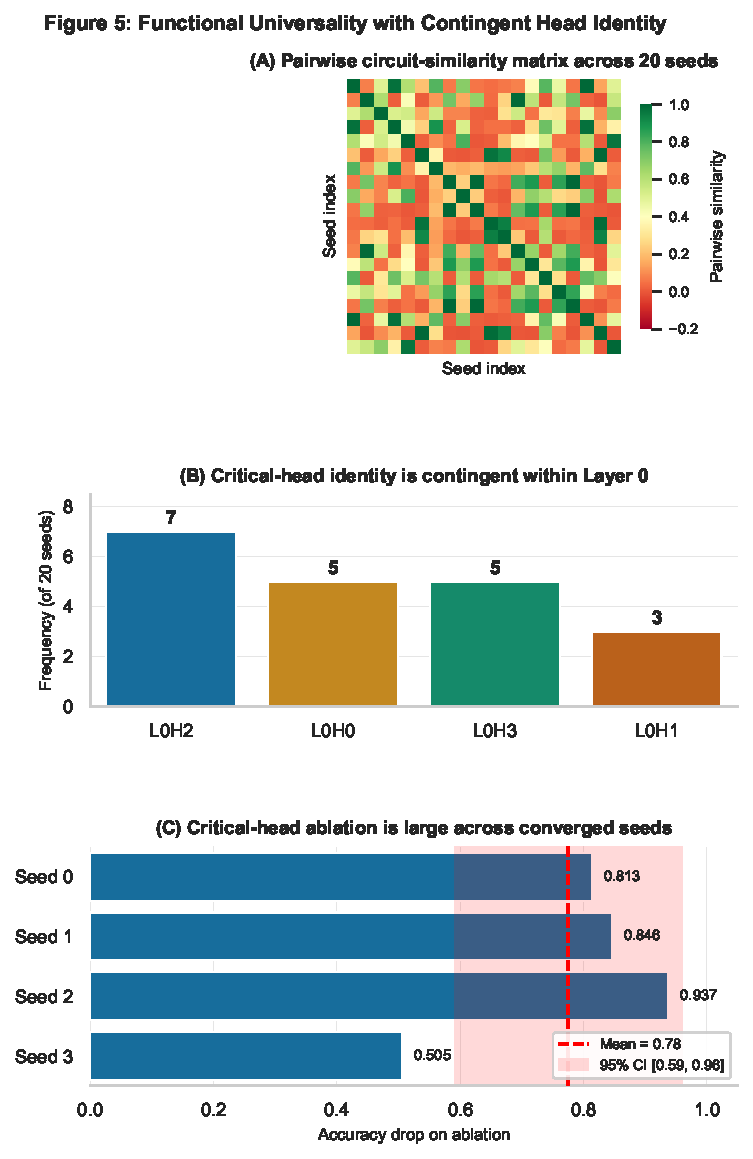
\includegraphics[width=\textwidth,height=0.72\textheight,keepaspectratio]{figures/fig5_universality.pdf}
  \caption{\textbf{Functional universality, structural contingency, weight
  direct weight non-portability.} (A) Pairwise head-level ablation effect similarity across
  20 seeds of the content-matching induction task (mean 0.329, CI [0.28, 0.38]).
  (B) Critical-head identity across 20 seeds: all 4 L0 heads receive the role
  (L0H0:5, L0H1:3, L0H2:7, L0H3:5); no L1 head does. Head-level
  agreement: 23.2\% ($p=0.002$ vs.\ random baseline 12.5\%). (C) Transplantation
  controls across all 4 seeds show consistent failure.}
  \label{fig:universality}
\end{figure}

%-----------------------------------------------------------------------
\section{Scale Probes: 19M Shakespeare and Pythia 160M}
\label{sec:scale}

The transplantation experiments above use 0.46M-parameter 2L/4H content-matching
induction models. To test whether non-portability holds at a larger scale on a
different task, we replicate the transplant protocol at 19M parameters
(6L/8H/d=512) on a TinyShakespeare character-level language model. We train
4 seeds (0--3) from scratch with different initializations but identical data;
seed 0's critical head is L0H7, while seeds 1, 2, 3 use different critical
slots, as in the 0.46M case. We transplant from seed 0 into each of 3
recipients and take the mean $\pm$ SD across recipients.

\begin{table}[h]
\centering
\small
\caption{Shakespeare 19M transplant vs.\ 0.46M content-matching induction. 19M
results are mean $\pm$ SD across 3 recipient seeds. At 19M on natural
language, single-head slot-matched transplant largely preserves induction
advantage. Functionally-matched cross-slot transplant still fails, including
after a redundancy-control that ablates other L0 heads while preserving the
recipient's critical slot. The core basis-dependence claim survives but with
scale/task-dependent quantitative strength.}
\label{tab:scale_replication}
\begin{tabular}{lcc}
\toprule
Transplant condition & 0.46M (induction) drop & 19M Shakespeare drop ($n=3$) \\
\midrule
Single-head slot-matched & 0.869 & \textbf{0.077 $\pm$ 0.038} \\
Function-matched single head & (same: 0.869) & \textbf{0.591 $\pm$ 0.022} \\
Slot-matched Procrustes & $\sim$0.88 & 0.125 $\pm$ 0.035 \\
Controlled critical-slot transplant & --- & \textbf{0.445 $\pm$ 0.040} \\
Controlled Procrustes & --- & 0.287 $\pm$ 0.029 \\
Whole L0 attention (all 8 heads) & 0.96 & 0.631 $\pm$ 0.029 \\
Full L0 block & 0.96 & 0.955 $\pm$ 0.029 \\
Full transplant (sanity check) & $\leq 0.11$ & 0.0 \\
\bottomrule
\end{tabular}
\end{table}

\paragraph{What changes at 19M.}
Slot-matched single-head transplant preserves $92\%$ of the induction advantage
on average, with tight variance across recipients (drops: 0.094, 0.032, 0.104
for recipients 1, 2, 3; mean 0.077 $\pm$ 0.038). At 0.46M, the same class of
transplant failed catastrophically. This is a real walk-back from a
scale-invariant reading of the small-model result. Two explanations are
plausible: (i) redundancy at scale --- 48 heads vs.\ 8 means each head is less
load-bearing, so substituting one is absorbed; (ii) the previous-token function
is simpler and more interchangeable than content-matching, so its weight
representation is more universal across seeds. Both explanations imply that
basis-dependence can weaken when scale, redundancy, and task change together.

\paragraph{What persists at 19M.}
Transplanting seed 0's critical head into each \emph{recipient's} critical slot
(functionally-matched, L0H7 $\to$ recipient's distinct head) drops advantage by
$0.591 \pm 0.022$ --- essentially catastrophic across all 3 recipients.
Whole-L0 attention transplant drops $0.63 \pm 0.03$; whole-L0 block drops
$0.96 \pm 0.03$. Wider transplants retain the coupling pattern we saw at 0.46M.
The 19M results refine rather than refute the core claim: basis-dependence is
present at both scales. At 19M, slot-matched single-head transplants escape
the coupling because the recipient doesn't critically depend on that slot;
functionally-matched cross-slot transplants, where the recipient's critical
computation \emph{is} being substituted, still fail --- with a 7.6$\times$
larger drop than slot-matched.

\paragraph{19M redundancy control.}
To distinguish redundancy from task-dependence, we run a second 19M control. For
each recipient, we search over subsets of non-critical L0 heads and select the
largest ablation set that preserves induction advantage above 0.50 while
keeping the recipient's own critical slot load-bearing. The selected controls
ablate 4 L0 heads on average, retain controlled advantage 0.520 $\pm$ 0.020,
and zeroing the critical slot under this control drops advantage by
0.449 $\pm$ 0.047. Transplanting seed 0's L0H7 into that load-bearing critical
slot drops advantage by 0.445 $\pm$ 0.040; Procrustes reduces but does not
remove the drop (0.287 $\pm$ 0.029). Thus the low slot-matched drop at 19M is
not sufficient evidence that the weights are portable. When the transplant is
forced through a recipient slot that the controlled host actually depends on,
non-portability remains large.

\paragraph{Pythia-160M scale probe.}
We also run a scale probe on the public Pythia-160M seed family:
six checkpoints, 15 cross-seed donor-recipient pairs, selected by attention to
the induction-relevant previous token on a synthetic induction prompt set. The
recipient baselines on this probe are lower than the small trained induction
models (0.0664--0.1426), but the selected heads are behaviorally relevant:
zeroing the selected recipient head reduces accuracy for every recipient.
Unaligned cross-seed transplantation drops below recipient baseline in all 15
pairs, with mean transplant-minus-baseline delta $-0.0589$. Two-interface
Procrustes also stays below baseline in all 15 pairs (mean delta $-0.0454$).
The broad all-four adapter condition reaches high accuracy, but so does the
zero-head adapter control; adapter accuracy is 0.819 on transplanted pairs and
0.834 for zero-head recipient controls. Therefore this Pythia adapter result is
not evidence that the donor head is being recovered. It shows that the frozen
Pythia backbone plus broad adapters can learn the synthetic probe, independent
of donor-head content (Table~\ref{tab:pythia160m}).

\begin{table}[h]
\centering
\small
\caption{Pythia-160M selected-head transplant probe. Comparable public 1.4B
multi-seed checkpoints were not available for a matched cross-seed test. Broad
adapters solve the synthetic probe, but the zero-head adapter control solves it
equally well.}
\label{tab:pythia160m}
\begin{tabular}{p{0.36\linewidth}cp{0.38\linewidth}}
\toprule
Quantity & Value & Notes \\
\midrule
Models & 6 & default + seed1--seed5 \\
Cross-seed pairs & 15 & all unordered pairs \\
Recipient baseline range & 0.0664--0.1426 & synthetic induction prompt set \\
Selected-head attention-score range & 0.4978--0.6920 & attention from second $A$ to first $B$ \\
Unaligned minus baseline & $-0.0589$ & all 15 pairs negative \\
Procrustes minus baseline & $-0.0454$ & all 15 pairs negative \\
All-four adapter accuracy & 0.819 $\pm$ 0.035 & transplanted pairs \\
Zero-head adapter accuracy & 0.834 & mean over recipient controls \\
\bottomrule
\end{tabular}
\end{table}

\paragraph{Scope.}
This is three recipient data points at 19M on one task family. A proper
frontier-scale test remains outstanding. The Pythia-160M result is a real
cross-seed scale datapoint from public checkpoints, but the recipient baselines are small
and the broad adapter rescue is not donor-specific. The nuance documented here
--- slot-matched Shakespeare transplant at 19M survives, redundancy-controlled
critical-slot transplant does not, Pythia-160M unaligned and Procrustes
transplants remain below baseline, and Pythia adapters require zero-head
controls --- argues against a scale-invariant binary claim. Portability is
scale-, task-, and interface-dependent.

%-----------------------------------------------------------------------
\section{Task Structure Determines Architecture}
\label{sec:taskarch}

\paragraph{Three regimes.}
Training identical model classes on different tasks produces qualitatively
distinct circuit architectures:

\begin{enumerate}
\item \textbf{Positional induction} (repeated-sequence, entropy=0): all heads
      positional; MLPs dominate logit attribution; trains in ${\sim}200$ steps.
\item \textbf{Content matching} (random-position bigrams): L1 heads
      develop content-based attention ($\mathtt{pos\_dep} \approx 0.70$); L1
      attention dominates logit attribution ($+18.96$); trains in ${\sim}13{,}000$
      steps via grokking-like delayed generalization; 60$\times$ cost gap vs.\
      positional.
\item \textbf{Natural language} (Shakespeare, high entropy): suppression cascade;
      Layer 0 encodes (7 copy heads + 1 previous-token head, score=0.908); layers
      1--5 progressively suppress wrong candidates; final MLP predicts; 39/48
      heads are content-based suppressors.
\end{enumerate}

\paragraph{Binary phase transition.}
Markov-chain models trained at 11 entropy levels (H=0.0 to H=1.0) reveal that
the architectural choice is \emph{binary}, not continuous. At $H=0$: 81\%
positional heads, attention functionally bypassed (zeroing all attention drops
accuracy only 1.5\%; zeroing all MLPs drops it 99.5\%). At any $H > 0$:
immediately switches to 75\% suppression + 25\% copy, stable from 0.5 nats to
4.1 nats. The threshold is the \textbf{attention-engagement threshold}: any
learnable uncertainty triggers attention; zero uncertainty bypasses it entirely.

This extends \citet{kawata2025shortcut}'s theoretical positional/content-matching
dichotomy to a three-regime empirical taxonomy, and reframes the binary
transition as ``attention-bypass vs.\ attention-active'' rather than
``positional vs.\ content-based.''

\begin{figure}[H]
  \centering
  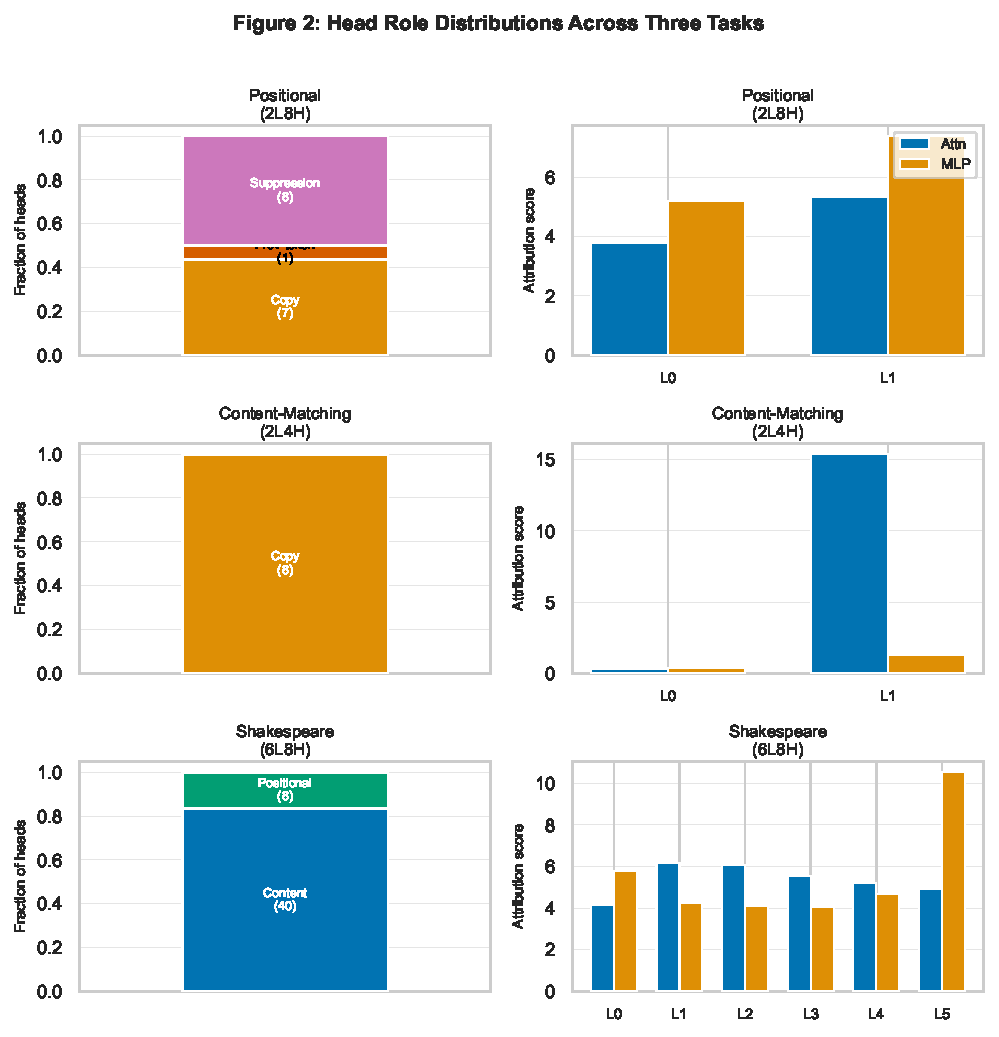
\includegraphics[width=\textwidth]{figures/fig2_architectures.pdf}
  \caption{\textbf{Task structure determines circuit architecture.} Three small
  transformers (same class, different tasks) develop qualitatively distinct
  architectures. Left: positional induction (MLP-dominant, 200 steps). Middle:
  content-matching induction (attention-dominant L1, grokking transition, 13,000
  steps). Right: Shakespeare character-level (suppression cascade, 6,000 steps).}
  \label{fig:threearchitectures}
\end{figure}

%-----------------------------------------------------------------------
\section{Developmental Order in Circuit Formation}
\label{sec:devorder}

We ask: does circuit formation follow a reliable temporal order?

\subsection{The grokking transition (content-matching induction)}

Training produces a striking delayed transition: task accuracy hovers near
chance for ${\sim}11{,}000$ steps, then jumps from 6\% to 85\% over
${\sim}1{,}000$ steps. We load 11 checkpoints spanning this window and measure
per-head OV copy score, QK content-matching score, and induction attention.

\begin{table}[h]
\centering
\small
\caption{Developmental timeline: content-matching induction model.}
\label{tab:grokking}
\begin{tabular}{p{0.23\linewidth}p{0.20\linewidth}p{0.47\linewidth}}
\toprule
Phase & Steps & Event \\
\midrule
Silent precursor     & 500--1,500    & OV copy scores rise across all heads \\
Extended plateau     & 1,500--12,000 & No QK movement, no accuracy change \\
Ignition             & 12,500        & QK content-matching crosses threshold \\
Crystallization      & 13,000--13,500 & L1 $\mathtt{pos\_dep}$ drops; L1$_\text{attn}$ attribution rises from $7.6$ to $12.9$; accuracy rises from $45\%$ to $75\%$ \\
\bottomrule
\end{tabular}
\end{table}

\textbf{The OV circuit becomes functional ${\sim}12{,}000$ training steps before
the QK circuit activates.} The model possesses the output capacity for induction
long before it acquires the routing capacity that makes output capacity useful.
We call this \textbf{``hardware before software.''} This finding is consistent
with \citet{singh2024induction}'s observation that QK matching is the
bottleneck, but we additionally identify the extended OV precursor as a distinct
detectable phase.

\subsection{Generalization across seeds (positional regime)}

We collect 81 dense checkpoints across each of 20 seeds of the positional
induction model and compute crystallization steps for four per-head metrics.
Pairwise orderings:
\begin{itemize}
\item copy-score before prev-token-score: 65\% of seeds
\item copy-score before induction-score: 80\% of seeds
\item copy-score before task-accuracy: 95\% of seeds
\end{itemize}
The copy-before-accuracy ordering is nearly universal (95\%), and
copy-before-prev-token-score holds in 65\% of seeds ($p < 0.001$ vs.\ random
ordering null at 4.2\%). The grokking-regime OV-before-QK ordering generalizes
as a directional trend, though the 12,000-step separation is specific to the
grokking regime.

\begin{figure}[H]
  \centering
  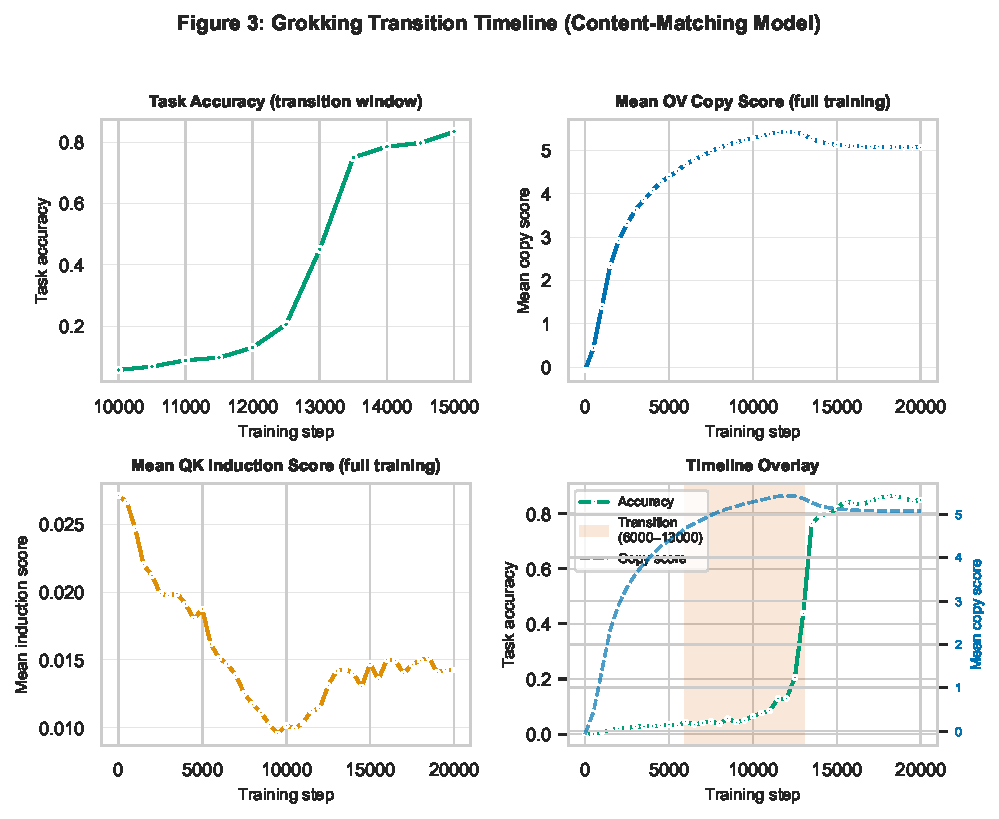
\includegraphics[width=\textwidth]{figures/fig3_grokking.pdf}
  \caption{\textbf{Hardware before software: output circuits form before routing
  circuits.} Training dynamics of the content-matching induction model across
  20,000 steps. (A) Accuracy: near-chance for 11,000 steps; sharp transition
  steps 12,500--13,500. (B) OV copy score: rises from step 500, reaches
  threshold by step 1,500. (C) QK content-matching score: flat until step
  12,500, then crosses threshold simultaneously with the accuracy transition. (D)
  OV crosses functional threshold ${\sim}11{,}000$ training steps before QK.}
  \label{fig:grokking}
\end{figure}

\subsection{Implication for capability monitoring}

The grokking-regime OV precursor is a large (${\sim}12{,}000$ step)
early-warning window. If this generalizes to capabilities in larger models that
form via grokking-like dynamics, OV-activity monitoring could anticipate
capability emergence during pretraining.

%-----------------------------------------------------------------------
\section{Depth Scaling of Suppression Cascades}
\label{sec:depth}

We train Shakespeare character-level models at depths 2, 4, 6, and 8 (all else
equal) to test whether the suppression cascade is a depth-scalable motif.

\begin{table}[h]
\centering
\caption{Suppression cascade increases approximately linearly with depth.}
\label{tab:depth}
\begin{tabular}{ccccccc}
\toprule
Depth & Eval loss & N supp. & \% supp. & N copy & N prev-tok & MLP/Attn ratio \\
\midrule
2 & 1.05 & 8/16  & 50\% & 7 & 1 & 8.56 \\
4 & 0.82 & 23/32 & 72\% & 7 & 1 & 9.35 \\
6 & 0.66 & 39/48 & 81\% & 7 & 2 & 9.02 \\
8 & 0.57 & 55/64 & 86\% & 7 & 1 & 9.08 \\
\bottomrule
\end{tabular}
\end{table}

\paragraph{Three universal facts across all depths.}
(1)~Layer 0 has zero suppression---reserved for copy heads (${\sim}7/8$) and
one previous-token head. (2)~Suppression grows monotonically with layer depth.
(3)~Peak suppression plateaus at ${\sim}2.0$ in the final layer.

\paragraph{Scaling trend.}
Across the four depths tested, the suppression fraction increases approximately
linearly with depth (OLS slope 0.059/layer,
$R^2 = 0.90$; 95\% CI [0.023, 0.109]).

\paragraph{MLP dominance persists across depths.}
Using direct logit attribution onto target tokens (rather than component output
L2-norms), MLPs dominate attention at every depth tested (ratios
$8.56\times, 9.35\times, 9.02\times, 9.08\times$ for depths 2, 4, 6, 8). An
earlier analysis using output norms showed an apparent attention--MLP crossover
at depth 8; that finding did not survive proper logit-attribution measurement
and is retracted here. The retained claim is the consistent magnitude-of-dominance
ratio: MLPs carry roughly an order of magnitude more direct logit contribution
than attention at every depth in our range.

\begin{figure}[H]
  \centering
  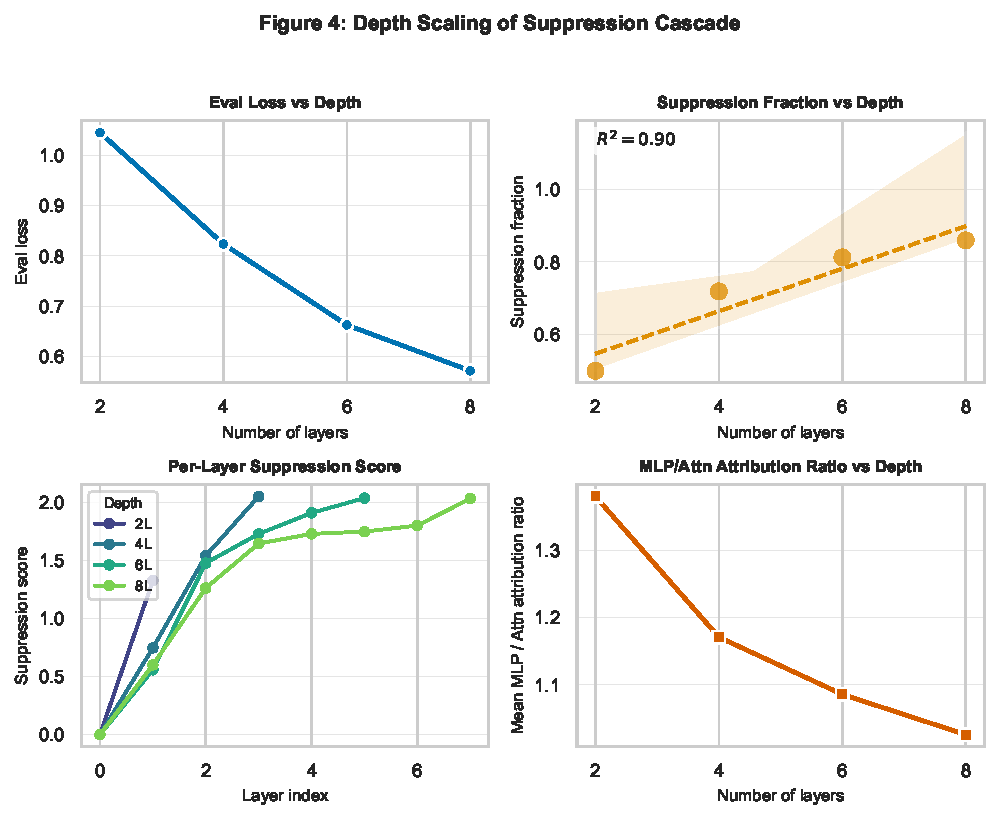
\includegraphics[width=\textwidth]{figures/fig4_depth_scaling.pdf}
  \caption{\textbf{The suppression cascade increases with depth.} Shakespeare
  character-level models at depths 2, 4, 6, 8. Top left: eval loss vs.\ depth.
  Top right: fraction suppression heads (OLS slope 0.059/layer, $R^2=0.90$).
  Bottom left: per-layer suppression scores---Layer 0 is always zero; suppression
  grows monotonically. Bottom right: MLP/attention direct logit attribution ratio
  is consistently ${\sim}9\times$ across all depths; MLPs dominate at every depth
  tested.}
  \label{fig:depthscaling}
\end{figure}

%-----------------------------------------------------------------------
\section{Natural Language Bridge}
\label{sec:nlp}

Circuits identified on synthetic tasks predict in-context copying behavior on
real language.

\paragraph{In-context copying in Shakespeare.}
On positions where a character bigram has already appeared earlier in context,
the Shakespeare model predicts the repetition with accuracy 1.000. The correct
null is not the uniform-chance 0.015 but the best non-induction baseline, which
is 0.292 (predict the most frequent character: space) or 0.076 (corpus-bigram
prediction). The induction advantage over the strongest baseline is
$1.000 - 0.292 = 0.708$. Ablating the identified induction heads (L0H7, L1H6,
L2H4) drops this advantage by 0.586---a large effect confirming these heads
drive the in-context copying behavior predicted by the synthetic-task circuit
maps.

\paragraph{L0H7: critical previous-token head.}
Ablating L0H7 alone, with previous-token score 0.908, raises eval loss from
0.080 to 7.95 ($\Delta = +7.87$)---worse than random initialization. This is a
large single-head ablation effect and identifies L0H7 as a load-bearing
previous-token head.

\paragraph{Suppression cascade is structural.}
Ablating layers 2--5 attention collectively raises loss by 5.08, confirming the
suppression cascade is causally necessary, not merely correlated with depth.

\paragraph{Careful framing.}
The previous-token head prediction generalizes cleanly from synthetic to natural
language. Two of the three content-matching head predictions do not drive large
individual effects on their own---at the character level, previous-token
attention dominates induction, with content-matching heads contributing
secondarily. This is consistent with \citet{olsson2022induction}'s analysis at
token level.

%-----------------------------------------------------------------------
\section{Discussion}
\label{sec:discussion}

\subsection{Circuits as computations, not modules}

Our transplantation and rescue results support a qualified reading:
\textbf{circuits are computations a self-organizing basis supports, not raw
components that can be moved without their interfaces}. The circuit---understood
as a functional description---can recur across networks computing the same
task; the specific weight matrices that realize it are basis-dependent. They
can become usable in a new host, but only after the host learns or is supplied
with the relevant compatibility map.

\subsection{Consequences for interpretability}

Our finding constrains interpretability methods that implicitly assume
portability:
\begin{itemize}
\item \textbf{SAE-based circuit discovery} produces basis-dependent features.
      Learned feature dictionaries should be treated as basis-dependent objects
      unless cross-run alignment has been explicitly validated.
\item \textbf{Circuit editing} may work within a network but should not be
      expected to transfer across models without adapter or retraining
      machinery.
\item \textbf{Claims of cross-model circuit universality} should be qualified:
      universality at the algorithm level, contingent implementation at the
      component level, and conditional portability at the weight level.
\end{itemize}

\subsection{Connection to the universality debate}

The Lan--Bali tension dissolves under our framing. Feature spaces are universal
in the sense that any sufficient basis supports the same computation---this is
what \citet{lan2025universal} measure across architectures. Individual heads are
unstable in the sense that within a given basis, many component-level
realizations are equally good---this is what \citet{bali2026headstability}
measure across seeds. Both observations are true; they do not conflict.

\subsection{Alignment and monitoring implications}

The developmental-order finding (Section~\ref{sec:devorder}) suggests OV
activity as an early-warning monitor for capability emergence: output capacity
is observable well before the capability it enables becomes functional. The
depth-scaling trend (Section~\ref{sec:depth}) documents that the suppression
cascade lengthens linearly with depth while Layer 0 composition remains
invariant (7 copy + 1 previous-token across all tested depths), suggesting the
``bottom of the network'' is a reliable encoding layer across trained character-level
language models.

\subsection{Toward a quantitative basis-mismatch metric}

The adapter results suggest a natural follow-up metric: the minimum description
length of a successful compatibility map. In the present paper we measure
whether fixed adapter classes rescue transplantation, not the minimal adapter.
A stronger follow-up would sweep adapter rank, sparsity, and placement across
many seed pairs and use the smallest successful map---in bits or trainable
parameters---as a quantitative basis-mismatch measure. The same framework would
also distinguish task-specific from task-agnostic portability by testing
cross-task transplantation with adapters, e.g.\ whether a content-matching head
can be made useful in a positional-induction host with only a learned
compatibility map.

%-----------------------------------------------------------------------
\section{Limitations}
\label{sec:limits}

\paragraph{Scale.} Most transplantation and rescue results use
$\sim$460K-parameter 2-layer models. We report one mid-scale replication on a
19M-parameter 6-layer character-level language model and one limited
Pythia-160M scale probe. These are not a substitute for a frontier-scale
suite: the 19M model is a character-level previous-token setting, the Pythia
probe uses a low-baseline synthetic induction task, and comparable public 1.4B
multi-seed checkpoints were not available for a matched cross-seed test. The
Pythia adapters also require a strong caveat: broad
all-four adapters solve the probe even when the selected head is zeroed, so the
Pythia adapter condition cannot be interpreted as donor-head rescue. Whether
the co-adaptation we document strengthens, weakens, or qualitatively changes at
larger scale is open.

\paragraph{Task diversity.} We study five task families. Transplantation is
tested only on content-matching induction. We have not tested whether whole-layer
transplantation across different training seeds also fails for IOI, modular
arithmetic, or other multi-component circuits.

\paragraph{Fixed data seed.} All seed-divergence experiments fix the data seed
and vary only model initialization. Co-variation of data and model seeds may
produce different universality statistics.

\paragraph{Statistical power.} Ablation robustness uses only 4 seeds (Appendix
\ref{app:ablation}). The head-level agreement statistic (23.2\%) has a wide
confidence interval [17.4\%, 29.5\%]. Deeper statistical characterization is
needed.

\paragraph{Alignment methods.} We test seven head-interface alignment methods spanning
orthogonal, affine, unconstrained linear, Git Re-Basin permutation matching
\citep{ainsworth2022git}, and learned nonlinear adapters
(Table~\ref{tab:alignment_tournament}). None rescues the head-local transplant;
the best method (nonlinear adapter) only reaches $0.118$ accuracy
(vs.\ $0.964$ baseline) by learning to ignore the donor head, matching
the donor-zero control at $0.1178$. Broader learned adapters do rescue
(Table~\ref{tab:stitching_adapters}), so the negative claim is limited to
raw transplants and head-local alignment, not to all possible compatibility
maps.

\paragraph{Partial retraining.} The partial-retraining rescue demonstrates that
the donor head contains usable structure, but it does not isolate which host
parameters learn the compatibility map. A follow-up should measure which
recipient tensors change during the first 100--500 rescue steps.

\paragraph{Permutation-sensitivity metric.} The permutation-sensitivity metric
is validated by agreement with ground truth on the entropy=0 model, but it may
be noisy in intermediate entropy regimes where partial positional structure
exists.

%-----------------------------------------------------------------------
\bibliographystyle{plainnat}
\bibliography{references}

%-----------------------------------------------------------------------
\appendix

\section{Methods in Detail}
\label{app:methods}

\subsection{Model architecture}

All small-scale experiments use a GPT-2-style decoder-only transformer:
\begin{itemize}
  \item \textbf{Ablation / transplant / 20-seed universality studies:}
        2 layers, 4 heads, $d_\text{model}=128$, $d_\text{ff}=512$,
        context length 64, vocabulary 512 (${\sim}460$K parameters). All
        20 content-matching induction seeds are trained under this
        configuration. Seed 2 additionally re-trained for 30{,}000 steps
        (from step\_030000) after failing to cross the grokking threshold
        at the default 20{,}000-step budget.
  \item \textbf{Entropy-continuum studies:} 4 layers, 4 heads, $d_\text{model}=128$,
        $d_\text{ff}=512$, context length 64 (Markov chains with varying entropy).
  \item \textbf{Shakespeare depth scaling:} 2/4/6/8 layers,
        8 heads, $d_\text{model}=512$, $d_\text{ff}=2048$, context length 128
        (${\sim}6.3$M--25.2M parameters). The 6-layer Shakespeare portability
        and redundancy-control runs use the same width with context length 256.
\end{itemize}

All models use pre-LayerNorm, learned positional embeddings, and tied
input/output embeddings. The unembedding matrix is the transpose of the
embedding matrix. Implemented in MLX 0.31.1 on Apple Silicon with Metal.

\subsection{Training details}

\begin{itemize}
  \item Optimizer: AdamW, $\beta_1=0.9$, $\beta_2=0.999$, $\epsilon=10^{-8}$
  \item Weight decay: 0.01 (small models), 0.1 (Shakespeare)
  \item Learning rate: cosine schedule from $3\times10^{-4}$ to $10^{-5}$
  \item Batch size: 64 (small models), 32 (Shakespeare)
  \item Checkpoints: every 25 steps (formation film), every 100 steps (standard)
  \item All training uses fixed data seed 42; model initialization seed varies
\end{itemize}

\subsection{Task specifications}

\paragraph{Positional induction.}
Sequence $= [\mathbf{a}_1 \ldots \mathbf{a}_{L/2} \mid \mathbf{a}_1 \ldots \mathbf{a}_{L/2}]$,
$L=64$, vocab=50. The model learns to copy the second half from the first half.
All positions in the second half are induction targets; the correct token is at
a fixed positional offset $L/2$. No content matching required.

\paragraph{Content-matching induction.}
$n_\text{bigrams}=6$ random token pairs $(A_i, B_i)$ placed at two random
positions each in a sequence of length 64. Vocab=512 (collision probability
$\approx 0.12$; essentially no random matches). The model must identify the
first occurrence of $A$ to predict $B$ at the second occurrence. No positional
shortcut possible.

\paragraph{Markov chain.}
Next-token prediction on sequences sampled from an ergodic Markov chain.
Transition matrix entropy $H \in \{0.0, 0.1, 0.2, \ldots, 1.0\}$ (nats, per
step). Vocab=64, seq\_len=64.

\paragraph{Shakespeare.}
Character-level next-token prediction on TinyShakespeare (1.1M characters, 65-char
vocabulary including punctuation and newlines). Training split: 90\%, validation
split: 10\%.

\subsection{OV and QK circuit measurement}

The OV score measures how strongly a head copies attended tokens into the
residual stream. For head $h$ in layer $\ell$:
\[
  \text{OV}_h = \frac{(W^O_h W^V_h E)_{ii}}{|(W^O_h W^V_h E)_{ij}|_{i \neq j}} \quad \text{(diagonal/off-diagonal mean ratio)}
\]
where $E$ is the token embedding matrix. A high ratio indicates strong
identity-preserving copy.

The QK content-matching score measures how sharply a head attends to tokens
with the same embedding as the query:
\[
  \text{QK}_h = \mathbb{E}_x \left[ \frac{\sum_j \mathbf{1}[\text{token}(j) = \text{token}(q)] \cdot \text{attn}_{h}(q, j)}{\sum_j \text{attn}_{h}(q, j)} \right]
\]

\subsection{Transplantation protocol}

For single-head transplantation, we copy the donor head's $W^Q$, $W^K$, $W^V$,
and $W^O$ slices, where $W^O$ denotes the output columns corresponding to the
target head. For whole-block transplantation, we additionally copy MLP weights
and LayerNorm parameters. For two-interface Procrustes alignment:
\begin{enumerate}
  \item \textbf{Pre-L0 LN interface} (what Q/K/V read from): collect
        activations $X_0, X_1 \in \mathbb{R}^{N \times d}$ at
        $\mathtt{ln1(embed + pos)}$ from both networks on $N$ shared inputs.
        Compute SVD: $X_0^\top X_1 = U \Sigma V^\top$.
        Set $R_{\mathrm{in}} = UV^\top$ (minimizes $\|X_0 R - X_1\|_F$).
        Apply $R_{\mathrm{in}}$ to the donor's $W^Q, W^K, W^V$.
  \item \textbf{Post-L0 residual interface} (what out\_proj writes into):
        collect activations $Y_0, Y_1 \in \mathbb{R}^{N \times d}$ after the
        first transformer block.
        Compute SVD: $Y_0^\top Y_1 = U' \Sigma' V'^\top$.
        Set $R_{\mathrm{out}} = U'V'^\top$.
        Apply $R_{\mathrm{out}}^\top$ to the donor's $W^O$ output columns.
  \item Insert the double-rotated head weights into the recipient network.
\end{enumerate}
The diagnostic $R^2$ is computed as $1 - \|X_0 R - X_1\|_F^2 / \|X_1\|_F^2$.

\subsection{Extended rescue protocols}

\paragraph{Partial retraining.}
For each donor-recipient pair, we transplant the donor critical head into the
recipient critical slot, freeze the transplanted head's Q/K/V/O weights, and
continue training all other recipient parameters on the original
content-matching induction task. We evaluate at cumulative checkpoints
$K \in \{0,100,500,1000,2000,5000,10000,20000\}$ and report
$K^\star$, the first checkpoint that reaches at least 80\% of the original
recipient baseline.

\paragraph{Stitching adapters.}
For adapter rescue, the transplanted recipient is frozen and only inserted
adapters are trainable. The post-L0 condition inserts one residual linear map
after block 0. The all-four conditions insert residual adapters before the
embedding stream, after L0, after L1, and before the unembedding. Linear
adapters are $d \times d$ maps; MLP adapters use hidden width $4d$. All adapter
conditions train for 2000 AdamW steps on the same induction distribution.

\paragraph{Shared-trajectory forks.}
For fork point $N$, one model is trained from the fixed initialization for
$N$ shared steps, cloned, and then the two branches continue to 20,000 steps
under different data-order seeds. Each fork point is evaluated with three
branch pairs.

\paragraph{Shared-basis training.}
Two models are trained jointly with the usual masked language-modeling loss
plus $\lambda(1-\mathrm{CKA})$ at post-L0 and post-L1 residual streams. We
sweep $\lambda \in \{0,0.01,0.1,1.0\}$ and evaluate task accuracy, residual
CKA, unaligned transplant accuracy, and two-interface Procrustes transplant
accuracy.

\paragraph{19M redundancy control.}
For each Shakespeare recipient, we identify the critical L0 head from the
single-head ablation sweep. We then search all subsets of the other seven L0
heads on a fixed 256-sample screening set and select the largest subset whose
ablation keeps induction advantage above 0.50 while keeping the critical slot
load-bearing by at least 0.25 advantage. The selected ablation set is then
evaluated on the full 1024-sample set for baseline, critical-slot zeroing,
unaligned critical-slot transplant, and Procrustes critical-slot transplant.

\paragraph{Pythia-160M probe.}
The Pythia probe uses the six public 160M seed-family checkpoints,
constructs synthetic induction prompts with repeated $A,B$ pairs, selects the
head with highest mean attention from the second $A$ to the first $B$, and
copies that head's GPT-NeoX Q/K/V/O slices into the recipient's selected head.
Two-interface Procrustes aligns the donor and recipient selected layers using
the selected layer's input-LayerNorm activations and post-layer residual
activations. The adapter condition freezes the recipient and trains four
zero-initialized residual linear maps: after token embedding, before the
recipient selected layer, after the selected layer, and before the unembedding.
Zero-head adapter controls use the same adapters with the selected recipient
head zeroed. Evaluation uses float32 during attention scans for numerical
stability.

%-----------------------------------------------------------------------
\section{Permutation-Sensitivity Metric Validation}
\label{app:permtest}

\paragraph{Definition.}
For head $h$, input $x = (t_1, \ldots, t_L)$, let $\pi$ be a random permutation
of the token vocabulary applied to all positions: for each batch we draw a
permutation $\pi$ of $\{0, \ldots, V-1\}$ and replace every token $x$ with
$\pi(x)$. Compute attention patterns $A(x)$ and $A(\pi(x))$, where
$\pi(x) = (\pi(t_1), \ldots, \pi(t_L))$ permutes token identities while
preserving absolute positions. The permutation sensitivity is:
\[
  \text{PS}_h = \mathbb{E}_{x, \pi} \left[ \|A_h(x) - A_h(\pi(x))\|_F \right]
\]

\paragraph{Validation.}
On the entropy=0 Markov model: $\mathtt{pos\_dep}$ classifies 16/16 heads as
positional; $\text{PS}$ classifies 16/16 heads as positional ($\text{PS} < 0.01$
for all heads). The two metrics agree on ground truth.

On Shakespeare (depth 6): $\mathtt{pos\_dep}$ classifies 47/48 heads as
positional. $\text{PS}$ classifies 9/48 as positional, resolving 39 false
positives. All 39 false-positive heads are in layers 1--5 (not layer 0). The
failure mode: by layer 1, the residual stream already encodes rich content
information, and content-conditional attention produces patterns with low
cross-input variance.

\begin{figure}[H]
  \centering
  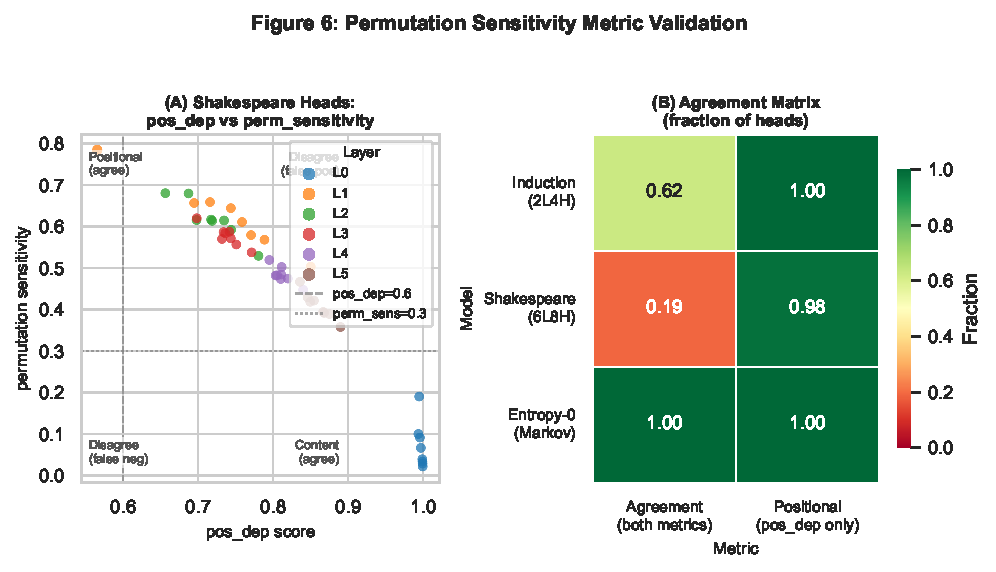
\includegraphics[width=0.9\textwidth]{figures/fig6_permutation_validation.pdf}
  \caption{\textbf{Permutation-sensitivity metric validation on Shakespeare.}
  Scatter of $\mathtt{pos\_dep}$ vs.\ permutation sensitivity $\text{PS}$ for
  all 48 attention heads in the depth-6 Shakespeare model. Only 9 heads are
  classified as positional by both metrics (bottom-left quadrant); 39 heads
  have high $\mathtt{pos\_dep}$ but high $\text{PS}$ (false positives under the
  old metric: content-based but pattern-stable). These 39 are concentrated
  in layers 1--5; Layer 0 (blue) heads largely agree.}
  \label{fig:permsens}
\end{figure}

%-----------------------------------------------------------------------
\section{Full Results Tables}
\label{app:results}

\subsection{Ablation robustness: four seeds}
\label{app:ablation}

\begin{table}[h]
\centering
\caption{Critical-head ablation across 4 seeds of the content-matching induction model. All critical heads are in Layer 0; specific head identity varies.}
\begin{tabular}{ccccc}
\toprule
Seed & Baseline accuracy & Critical head & Accuracy after ablation & Drop \\
\midrule
0 & 0.854 & L0H3 & 0.041 & \textbf{0.813} \\
1 & 0.964 & L0H1 & 0.118 & \textbf{0.846} \\
2 & 0.965 & L0H1 & 0.028 & \textbf{0.937} \\
3 & 0.968 & L0H3 & 0.463 & \textbf{0.505} \\
\midrule
\multicolumn{4}{l}{Mean drop} & \textbf{0.775 $\pm$ 0.162} \\
\bottomrule
\end{tabular}
\end{table}

\subsection{Bootstrap confidence intervals}

\begin{table}[h]
\centering
\caption{Statistical summary of key claims.}
\begin{tabular}{lcccl}
\toprule
Claim & Point estimate & 95\% CI & Null & $p$-value \\
\midrule
Layer-level agreement (20 seeds)   & 100\%     & [100\%, 100\%] & 50\%    & $<0.001$ \\
Head-level agreement (20 seeds)    & 23.2\%   & [17.4\%, 29.5\%] & 12.5\% & 0.002 \\
Head-level similarity (20 seeds)   & 0.329    & [0.28, 0.38]   & 0       & $<0.001$ \\
Ablation drop (4 seeds)            & 0.775    & [0.59, 0.91]   & 0       & 0.004 \\
Suppression slope (n=4 depths)     & 0.059/layer & [0.023, 0.109] & 0    & 0.052 \\
\bottomrule
\end{tabular}
\end{table}

%-----------------------------------------------------------------------
\section{Ablation Protocols}
\label{app:ablation_proto}

\paragraph{Zero-ablation.}
We zero-out a component's output by setting its contribution to the residual
stream to the zero vector. This is the least assumption-dependent ablation: it
tests whether the component's \emph{contribution} is necessary, without assuming
a particular ``baseline'' activation.

\paragraph{Critical-head identification.}
For each model, we identify the critical head as
\[
h^\star = \arg\max_h \left(\text{accuracy}_\text{baseline}
  - \text{accuracy}_{h\text{-ablated}}\right).
\]
We verify that this single head accounts for the majority of the model's
induction ability by checking that the remaining accuracy after ablation is near
the ablated-model floor ($\approx 0.09\text{--}0.12$ for 2L/4H
content-matching models), far below the functional baseline of $\approx 0.96$.

\paragraph{Transplantation ablation.}
In the clean-slate transplant condition, we zero the recipient's critical head before inserting the donor head. This tests whether the donor head can function even without the recipient's critical-head initialization (ruling out residual activation from the original weights).

\end{document}
